\chapter{Projektplan}

\section{Projektverknüpfungen}

Das Projektteam hat sich dazu entschlossen das Projekt über \gls{GitHub} zu verwalten. \\
Dort sind in einem \gls{Kanban-Board} alle Tasks des aktuellen \gls{Sprint}s und der abgeschlossenen \gls{Sprint}s zu finden. Alle Tasks die eine konkrete Arbeit erfordern sind einem \gls{Issue} zugeordnet. Dieses \gls{Issue} wird dann mit dem, den Task erfüllenden \gls{Pull-Request} verbunden. \\
Im \gls{Issue} ist auch das zuständige Projektteam für diese Aufgabe gekennzeichnet.\\
Für eine Übersicht der Projektverknüpfungen wird daher auf das \href{https://github.com/LucRome/SWE_Semester4/}{GitHub-Repository} und darin auf die \href{https://github.com/LucRome/SWE_Semester4/issues}{Issue-Liste} und das \href{https://github.com/LucRome/SWE_Semester4/projects/1}{Kanban-Board} verwiesen.
\section{Eskalationspfade}
Da dieses Projekt in keine gewöhnliche unternehmensinterne hierarchische Organisation eingebettet ist, können keine weitreichenden Eskalationspläne erstellt werden. In Abbildung \ref{fib:Eskalationspfad} ist dennoch ein kurzer graphischer Weg zum Umgang mit Problemen dargestellt. Dieser zeigt einen Weg auf, über den es möglich ist teamintern mit Problemen umzugehen.\\

\begin{figure}[h]
\centering
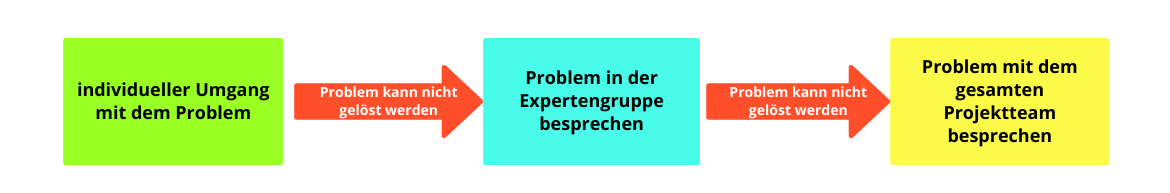
\includegraphics[height=.18\textwidth]{Eskalationspfad.png}
\caption{Eskalationspfad im Projekt eCourse}
\label{fib:Eskalationspfad}
\end{figure}

\section{Projektablauf}

\label{sec:ablauf}
Die Arbeit am Projekt startet startet am 18.03.2021 und endet am 20.05.2021. \\
Teamintern wurde festgelegt, dass die Projektorgansisation agil mittels \gls{Scrum} erfolgen soll.\\
Dies sieht vor, dass das Projekt in einzelne Entwicklungsstufen unterteilt ist, welche Iterationen genannt werden.\\
Zu Beginn wurden für den Scrum Prozess die drei Scrum-Rollen im Team verteilt. Die genaue Aufteilung der Rollen ist der Abbildung \ref{fib:Organigramm} zu entnehmen. \\
In Abbildung \ref{fib:Organigramm} ist ebenfalls zu sehen, dass das \gls{Development Team} nochmals aufgeteilt ist, in ein \gls{Frontend} und ein \gls{Backend} Team. Diese Maßnahme wurde durchgeführt, um für die beiden großen Themengebiete jeweils eine Expertengruppe zu bilden. Dadurch muss nicht jeder Entwickler mit allen Projektdetails vertraut sein, sondern nur mit seinem spezielleren Themengebiet. Ebenfalls wird dadurch die Verteilung von Tasks einfacher, da die Tasks dann in erster Linie dem Expertenteam zugeordnet wird und dort dann intern die Tasks noch weiter aufgeteilt bzw. verteilt werden können. \\
Die Dokumentation des Projektes wurde separat an ein Teammitglied ausgelagert. Dies gibt den \gls{Development Team} die Möglichkeit sich vollständig um die Implementierung neuer Features zu kümmern.\\
Der Scrum-Prozess wird im Team nach folgenden Regeln gestaltet:
\begin{itemize}
\item Jeder Sprint dauert genau eine Woche. Die Sprintlänge ergibt sich daraus, dass das Projekt sehr dynamisch ist und durch die beiden Expertenteams ein hohes Maß an Kommunikation erforderlich ist. Außerdem erlaubt die kurze Sprintdauer eine hohe Abhängigkeit zwischen den Tasks der beiden Gruppen.
\item \gls{Daily Scrum}s finden jeden Montag und Mittwoch statt. Eigentlich werden \gls{Daily Scrum}s an jedem Arbeitstag durchgeführt, allerdings ist es in diesem Projekt so, dass die einzelnen Teammitglieder nicht zu 100\% an diesem Projekt arbeiten. Dadurch werden nicht an jedem Arbeitstag neue Projektergebnisse generiert, über die gesprochen werden könnte. 
\item Der iterative Scrum-Prozess ist in Abbildung \ref{fib:Scrum} kurz dargestellt.
\end{itemize} 

\begin{figure}[h]
\centering
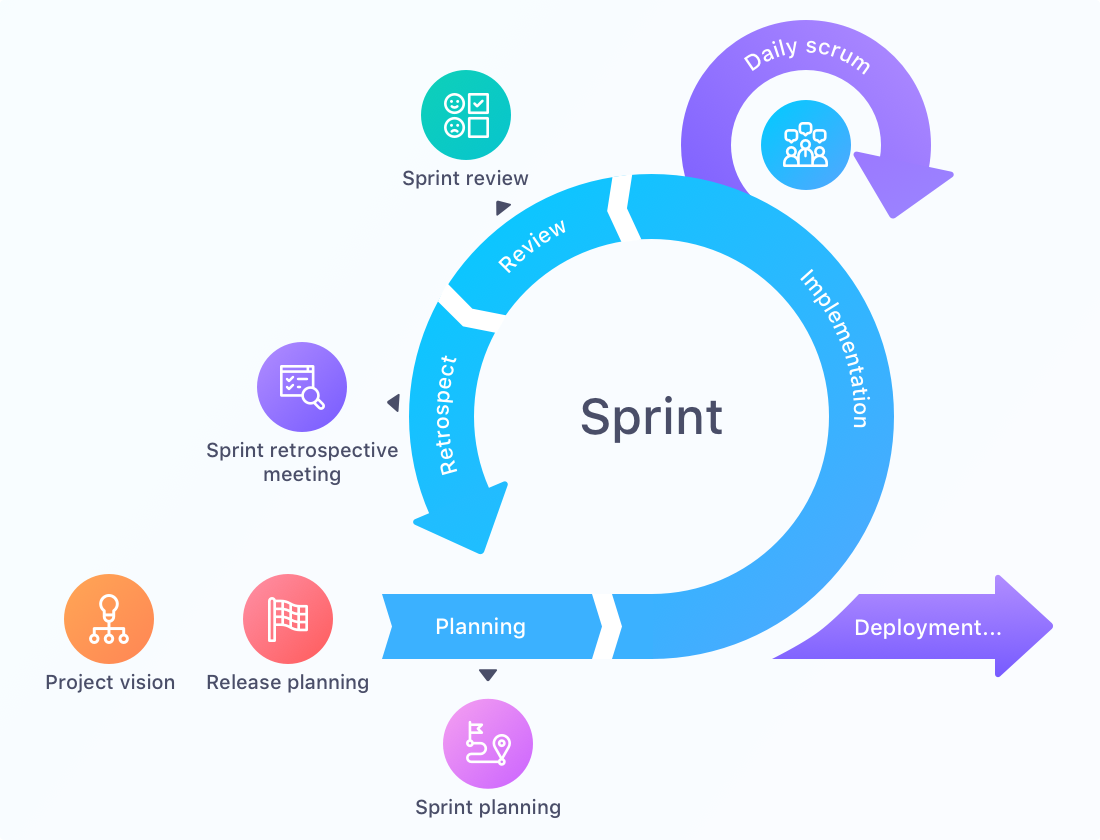
\includegraphics[height=.8\textwidth]{Scrum_Pic.png}
\caption{Scrum Prozess}
\label{fib:Scrum}
\end{figure}

\section{Meilensteinplan}

Wie im vorherigen Unterkapitel \ref{sec:ablauf} bereits erläutert, wird dieses Projekt agil entwickelt. Dadurch ergeben sich im Projekt keine Meilensteine.